\problemname{Guessing Game}
In the old town of Lund, there is a street with $N$ houses in a row, indexed
$0$ to $N-1$. Emma lives in one of these houses and her friends Anna and Bertil
want to figure out which one. Instead of just telling her friends where she
lives, Emma decides to play a game with them. 
Before the game starts, Anna and Bertil only know the number of houses on the street.
At this point, Anna and Bertil may pick a positive integer $K$ and agree on a strategy.
Any communication thereafter is forbidden.

The game itself consists of two phases. In the first phase, Emma picks 
an order in which to visit the houses, such that her house is the last one to visit.
She then leads Anna to the houses one by one in this order, without telling Anna the order in advance. 
For each house that is not Emma's house, Anna is allowed to write a single integer between $1$ and $K$ 
on the front door of the house with a piece of chalk. 
For the last house they visit, Emma's house, Emma writes an integer between $1$ and $K$ on the door herself. 

In the second phase of the game, Bertil walks along the street from house $0$ to house $N-1$ and reads all the numbers written 
on the doors by Anna and Emma. He now wants to guess which house Emma lives in. 
He has two chances to guess correctly and he and Anna win the game if he succeeds. Otherwise, Emma wins the game. 


Can you devise a strategy where Anna and Bertil are guaranteed to win the game?
Your strategy will be scored based on the value of $K$ (the smaller, the better).

\section*{Implementation}
This is a multi-run problem, meaning that your program will be executed multiple times.
The first time it is run, it will implement Anna's strategy. After that it will implement Bertil's.

The first line of the input will contain two integers, $P$ and $N$, where $P$ is either $1$ or $2$ (first or second phase),
and $N$ is the number of houses.
\textbf{Except for the sample input (not used for scoring), $N$ will always equal $100\,000$}.

The following input depends on the phase:

\subsection*{Phase 1}
Your program should start by outputting the number $K$ on a single line $(1 \le K \le 1\,000\,000)$.
Then, $N - 1$ times, it should read a line containing an index $i$ $(0 \le i < N)$, and output a line with an integer
 $A_i$ $(1 \le A_i \le K)$, where $A_i$ is the number Anna writes on the door of house $i$. 
 Every index $i$ except the index of Emma's house will appear exactly once, in some order decided by the grader.

\subsection*{Phase 2}
Your program should read a line with $N$ integers, $A_0, A_1, \ldots, A_{N-1}$, 
where $A_i$ is the number written on the door of house $i$.

Then, it should print a line with two integers, $s_1$ and $s_2$ $(0 \le s_i < N)$, the guessed indices.
$s_1$ and $s_2$ are allowed to be equal.

\subsection*{Implementation Details}

Note that when running your program in Phase 2, the program is restarted. 
This means that you cannot save the information in some variables between the runs. 

After each line you print, make sure to flush standard output, or else your program might get judged as Time Limit Exceeded.
In Python, \verb|print()| flushes automatically. In C++, \verb|cout << endl;| also flushes in addition to printing a newline; 
if using printf, use \verb|fflush(stdout)|.

The grader for this problem may be \textbf{adaptive}, meaning it may change its behavior depending on the output 
of your program to prevent heuristic solutions from passing.
It might do a trial run of phase 1, look at your output, and then run phase 1 for real using 
information it extracted from the previous run. 


\textbf{Your program \emph{must} be deterministic}, that is behave the same if run twice on the same input.
If you want to use randomness in your program, make sure to use a fixed random seed.
This can be done by passing a hard-coded constant to \verb|srand| (in C++) or \verb|random.seed| (in Python), 
or, if using C++11's random number generators, by specifying the seed when constructing the random number generator. 
In particular, you can not use \verb|srand(time(NULL))| in C++.
If the grader detects that your program is not deterministic, it will be given a Wrong Answer verdict.

If the \emph{sum} of the runtimes of the (up to $3$) separate runs of your program exceeds the time limit, 
your submission will be judged as Time Limit Exceeded.

\section*{Scoring}
Your solution will be tested on a number of test cases.
If your solution fails on \emph{any} of these test cases (e.g. by giving wrong answers (Wrong Answer), crashing (Run-Time Error), exceeding the time limit (Time Limit Exceeded), etc.), 
you will receive $0$ points and the appropriate verdict.

If your program successfully finds the index of Emma's house in \emph{all} test cases, you will get the verdict Accepted, and a score calculated as follows.
Let $K_{max}$ be the maximum value of $K$ used for any test case. Depending on $K_{max}$:

\noindent
\begin{tabular}{| l | l | l |}
\hline
                                & Score  \\ \hline
            $K_{max} > 99\,998$ & $10$ points  \\ \hline
$10\,000 < K_{max} \le 99\,998$ & $10 + \lfloor 40 (1 - K_{max} / 10^5) \rfloor$ points  \\ \hline
$30 < K_{max} \le 10\,000$      & $46 + \lfloor 31 (4 - \log_{10}(K_{max})) / (4 - \log_{10}(30)) \rfloor$ points  \\ \hline
     $7 < K_{max} \le 30$       & $107 - K_{max}$ points  \\ \hline
      $K_{max} \le 7$           & $100$ points  \\ \hline
\end{tabular}

The scoring function is depicted in the figure below.

\begin{center}
      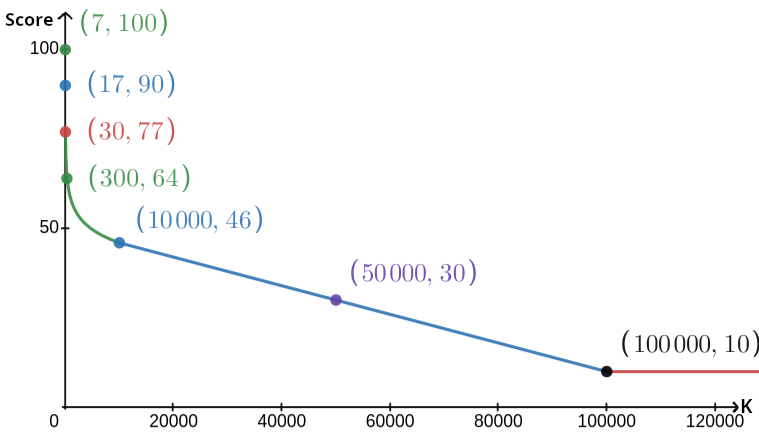
\includegraphics[width=.8\textwidth]{guessing-score-4}
\end{center}
    
The sample test case is ignored for scoring, and your solution does not have to work for it.

\section*{Testing Tool}

To facilitate the testing of your solution, we provide a simple tool that you can download.
See ``attachments'' at the bottom of the Kattis problem page.
The tool is optional to use, and you are allowed to change it. Note that the official grader program on Kattis is different from the testing tool.

Example usage (with $N=4$, $s=2$, where $s$ is the number written on the last house visited):

For Python programs, say \verb|solution.py| (normally run as \verb|pypy3 solution.py|):

    \verb|python3 testing_tool.py pypy3 solution.py <<<"4 2"|

For C++ programs, first compile it
(e.g. with \verb|g++ -g -O2 -std=gnu++17 -static solution.cpp -o solution.out|)
and then run:

    \verb|python3 testing_tool.py ./solution.out <<<"4 2"|

The testing tool will visit the houses in random order.
To use a specific order, modify the testing tool where it says ``MODIFY HERE''.

\section*{Example Interaction}

The sample test case is ignored for scoring, and your solution does not have to work for it.

Suppose we have $N = 4$ and that Emma lives in house $1$. 
Let $A$ be the list of numbers written on the houses.
Initially, $A = [0, 0, 0, 0]$, where $0$ means that no number is written on the corresponding house.

In the first run of your code:

$N = 4$ is given. Solution responds with $K = 3$.

$A_2$ is asked for. Solution responds with $3$. $A$ is now $[0, 0, 3, 0]$.

$A_0$ is asked for. Solution responds with $1$. $A$ is now $[1, 0, 3, 0]$.

$A_3$ is asked for. Solution responds with $2$. $A$ is now $[1, 0, 3, 2]$.

Finally, the grader sets $A_1 = 2$, so that $A = [1, 2, 3, 2]$ in the end.
This marks the end of the first phase.

In the Phase 2 of your code, the solution is passed the list \texttt{1 2 3 2}.

It responds with \texttt{1 3}.

Since one of the guesses is the correct index of the house $(1)$, Anna and Bertil win the game.
